\subsection{Components}

Figure \ref{fig:comp_dia} shows a high level view of the logical layout of the components in the MDApp.

\begin{figure}[H]
    \centering
    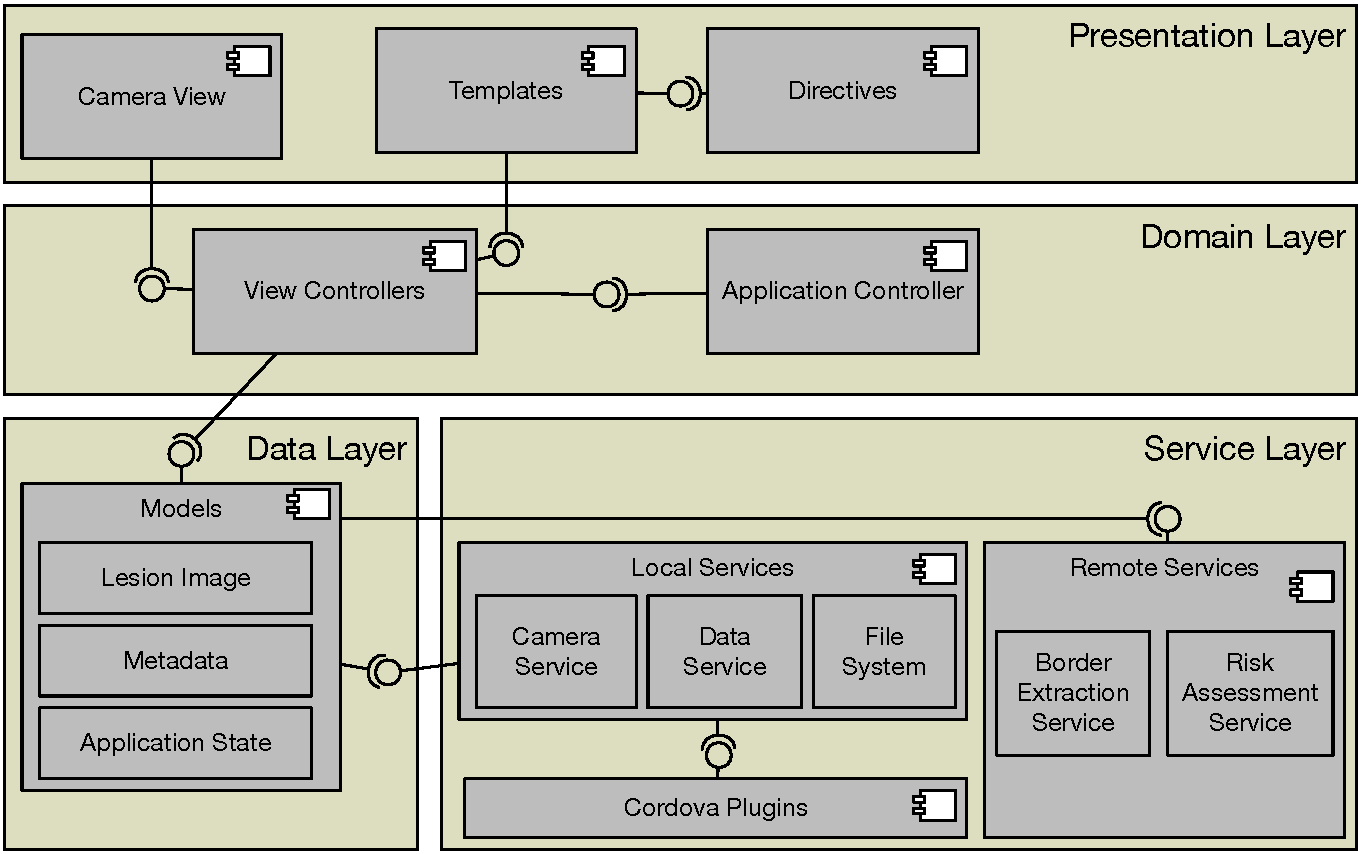
\includegraphics[width=\textwidth,keepaspectratio]{assets/architecture/compontent_diagram.pdf}
    \caption{Component diagram of the MDApp}
    \label{fig:comp_dia}
\end{figure}

\subsubsection{View Controllers}

Each view controller class is responsible for a specific view or partial view of the MDApp. In larger applications there might be multiple view controllers per “page” in a nested hierarchy. The MDApp will only require one controller per page, these are the HomeController, CameraController, AnalysisController and the ArchiveController. Each controller is responsible for preparing the data that will be displayed in the view as well as capturing and processing user events.

\subsubsection{Application Controller}
The application controller is a global controller that can manage the state of the app. It makes sure that the state is persevered when the MDApp is closed and restarted. It can also switch the user automatically from one view to another when appropriate or enable or disable the user interface when some activity is in progress.

\subsubsection{Templates, Directives and Camera View}
Except for the the Camera View all of the pages are created from HTML files that have prepared placeholders called directives. Directives are special markers in the HTML that the Angular framework uses to inject data and specific behaviour into the HTML element. Directives bundle together often used patterns into easily configurable markers that can be embedded into an HTML file.

The Camera View is an exception in the MDApp. The CameraView is an HTML template that overlays a realtime preview of the camera’s input. The realtime preview is not part of the Cordova/Phonegap browser view, it is a platform native view element that is provided by a 3rd party plugin. The cordova-plugin-camera-preview is a crossplatofrm wrapper around native code that allows the browser based javascript to communicate and control the camera preview view.

\subsubsection{Models}
The Models are relatively simple data classes. The MDApp does not require much buisiness logic for the data. The Models encapsulate some communication with some of the services so that the controllers can remain as simple as possible.

\subsubsection{Local Services}
The local services classes are just wrappers around the Cordova plugins. Cordova plugins offer a "raw" javascript API. The service classes will hide some of the complexity by making only the relevant functions available to the MDApp.

\subsubsection{Remote Services}
The remote services leverage the angular \$resource factory which provides easily configurable RESTful communication to online servers.

\subsubsection{Cordova Plugins}

In a hybrid architecture most of the logic is programmed in javascript, just like a normal web page. Communication with native system components and hardware APIs that a normal browser based environment does not have access can be enabled through plugins. Ideally these plugins unify the native APIs across all platforms. The MDApp uses the following cordova plugins:

   \paragraph{cordova-plugin-camera-preview}
   Several camera plugins exist for Cordova, however none of them allow a live camera preview to be embedded in the UI directly. Most pass the user to a native camera view. This makes it impossible for any UI components to be superimposed over the camera view. The cordova-plugin-camera-preview makes this possible by creating a native view component that can be positioned over or under the Cordova browser view. In order to overlay and components in the Cordova browser over the camera, the Cordova browser background must be made transparent. This can be done by setting the background of the html, body and some ionic components transparent.

   \paragraph{cordova-plugin-file-transfer}

   This plugin allows javascript running in the Cordova browser context to interface with a collection of native classes that manage file downloads and uploads.

   \paragraph{Cordova-sqlite-storage}

This plugin creates and manages connectivity to a local sqlite database file that is not subject to the limitations of a browser based file storage. Queries are faster, the storage capacity is much larger, and most importantly data will survive an application restart and update. A backup of the sqlite database file can be made using standard native backup strategies. This is not possible using the built in Cordova browser based data storage


\subsection{Classes}

The class diagram in figure \ref{fig:class_dia} shows the structure and connections between the main classes of the MDApp. The service layer classes are singletons that encapsulate the functionality of some plugin into an easy to manage form. Static class level methods and attributes are underlined. The other methods and attributes have object level scope.

\begin{figure}[H]
    \centering
    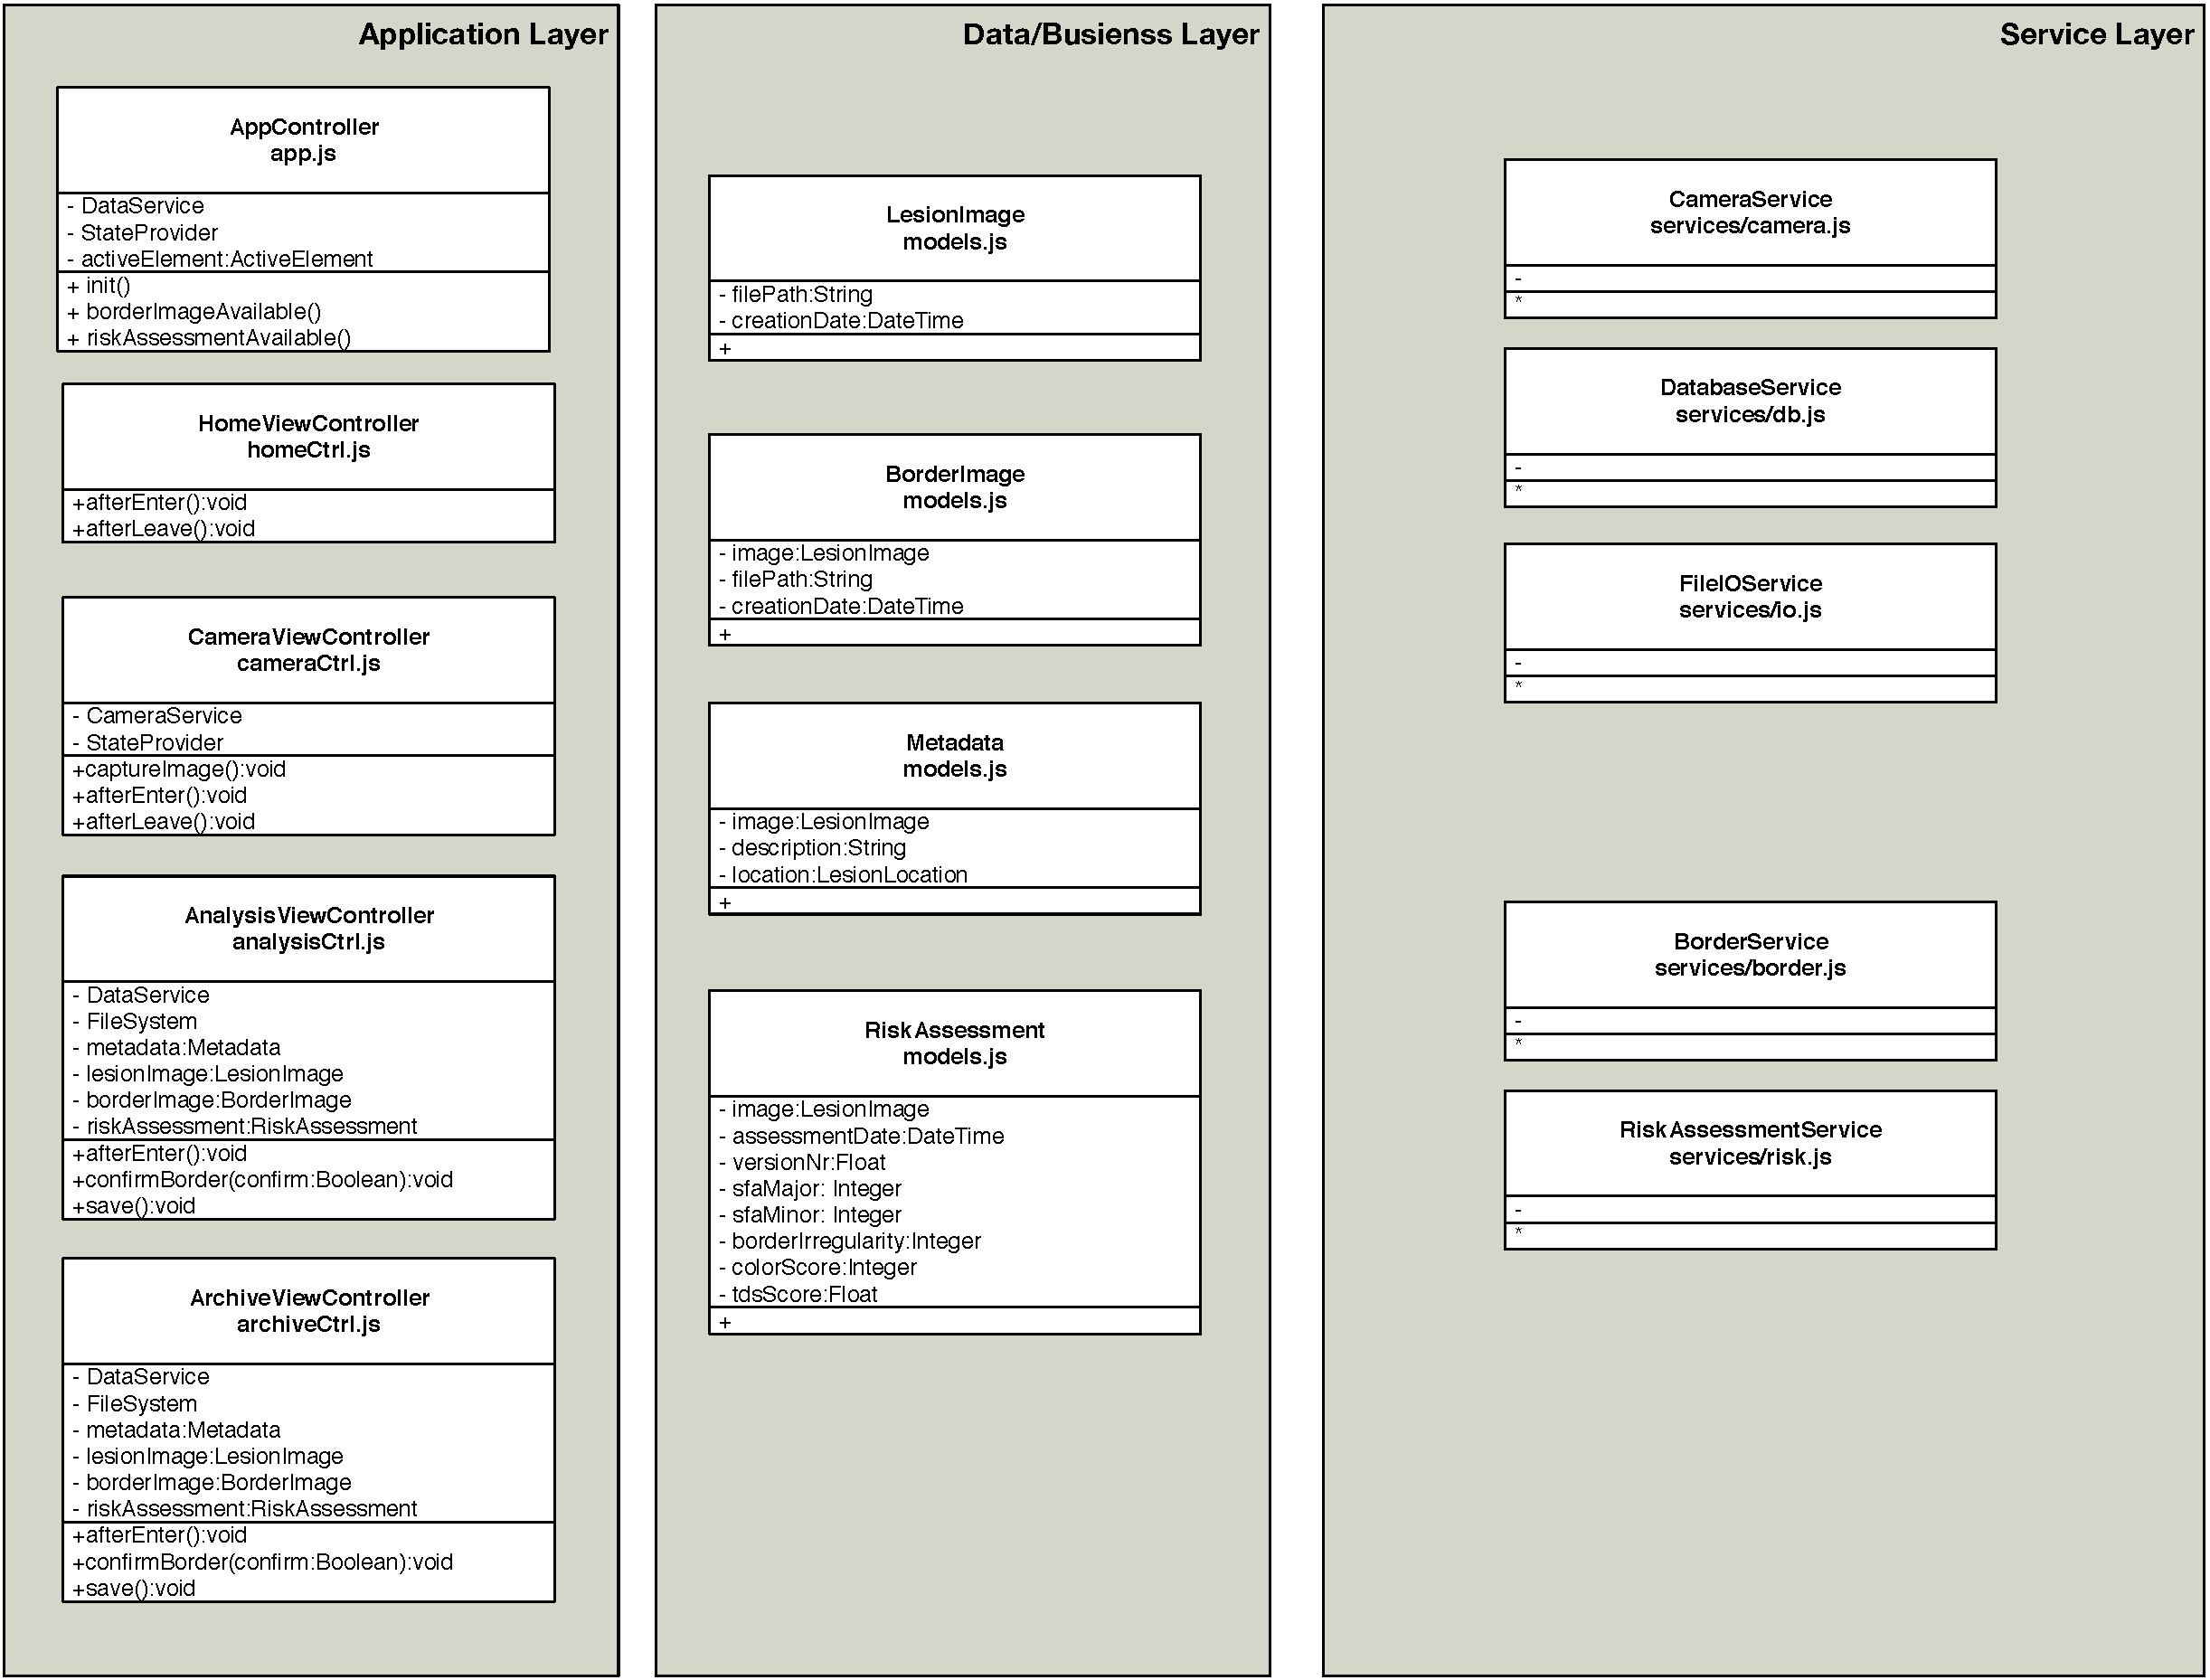
\includegraphics[width=\textwidth,keepaspectratio]{assets/architecture/class_diagram.pdf}
    \caption{Component diagram of the MDApp}
    \label{fig:class_dia}
\end{figure}

    \subsubsection{Application Layer}
        \paragraph{AppController}
                            \begin{longtable}[H]{  | >{\bfseries}l | l | l | l | l | }

                    \hline

                    Name
                    & \multicolumn{4}{l |}{AppController} \\ \hline

                    Description
                    & \multicolumn{4}{p{8.5cm} |}{The AppController manages the global state of the app. It can disable UI elements when the app needs to wait for longer processes. It can restore the previous state of the app after it has been reopened or updated.} \\ \hline

                    Type
                    & \multicolumn{4}{l |}{Class}
                    \\ \hline

                    Implemented In
                    & \multicolumn{4}{l |}{app.js}
                    \\ \hline

                    Attributes
                    & Name & Type & \multicolumn{2}{p{6.5cm} |}{Description} \\ \hline
                        & \$state & class & \multicolumn{2}{p{6.5cm} |}{
                        The \$state object is provided by the angular ui-router and is used to define pages in the app. It can be used to query or set the ui state. The AppController uses the \$state to automatically move the user from the camera view to the analysis view when the border data has become available, for example.
                        } \\ \hline
                        & MDAppState & class & \multicolumn{2}{p{6.5cm} |}{
                        The MDAppState stores data the the AppController might need to restore it's state after a restart.
                        } \\ \hline
                        & uiDisabled & boolean & \multicolumn{2}{p{6.5cm} |}{
                        This variable is used to trigger changes in the ui. Through 2-way binding the ui components in the view will become disabled or enabled respectivly.
                        } \\ \hline
                        & tabStates & object & \multicolumn{2}{p{6.5cm} |}{
                        This javascript object stored the disabled-state of the individual tab components in the ui. The AppController disabiles or enables specific tab elements based on the state of the app and the data currently available.
                        } \\ \hline


                    Methods
                    & Name & Parameter & Return Type & Description \\ \hline

                        &


                \end{longtable}
        \paragraph{CameraViewController}
            \footnotesize{
\begin{longtable}[H]{  | >{\bfseries}l | p{1.5cm} | p{1.5cm} | p{1.5cm} | p{4cm} | } \hline

    Name
    & \multicolumn{4}{l |}{CameraViewController} \\ \hline

    Description
    & \multicolumn{4}{p{8.5cm} |}{
    The CameraViewController manages the camera preview user interface. It received a user “tap” event from the view and triggers the image capture process. Because the actual camera view ui element is a native view element outside of and behind the Cordova browser view, specific ui components must be made transparent to let the camera view become visible. The CameraViewController activates this transparency when it is loaded and deactivates it when unloaded.

    } \\ \hline

    Type
    & \multicolumn{4}{l |}{Class}
    \\ \hline

    Implemented In
    & \multicolumn{4}{l |}{controllers/camera.js}
    \\ \hline

    Attributes
    & Name & Type & \multicolumn{2}{l |}{Description} \\ \hline

        & MDCameraService & class & \multicolumn{2}{p{5.5cm} |}{
        The CameraViewController passes the capture request from the user to the MDCameraService. The MDCameraService is also responsible for starting and stopping the camera preview.
        } \\ \hline
        & MDLesionImage & class & \multicolumn{2}{p{5.5cm} |}{
        When a new image is captured the CameraViewController notifies the MDLesionImage class which creates a new MDLesionImage instance.
        } \\ \hline
        & MDAppState & class & \multicolumn{2}{p{5.5cm} |}{
        When a new image is captured, the CameraViewController notifies the MDAppState that a new image is the active image.
        } \\ \hline


    Methods
    & Name & Parameter & Return Type & Description \\ \hline

        & captureImage & void & void
        & This method is triggered by the user and passed from the view to the view controller. The event is passed on to the MDCameraService along with a reference to the captureImageCallback which is called when an image has been saved.
        \\ \hline
        & captureImageCallback & results & void
        & The MDCameraService notifies the CameraViewController that an image is availble via this callback. The results parameter is a javascript object that contains a path to the captured image file and a preview image file.
        \\ \hline
        & afterEnter & void & void
        & When the camera view is loaded this method is called by the angular ui-router. The CameraViewController maked selected background UI components transparent in order to allow the camera preivew view to become visible.
        \\ \hline
        & afterLeave & void & void
        & The angular ui-router notifies the CameraViewController via this method that the user has moved to another view. The CameraViewController cleans up the transparent UI compontent, making them opaque.
        \\ \hline


    \caption{CameraViewController Specification}
    \label{fig:camera_controller}
\end{longtable}
}
        \paragraph{AnalysisViewController}
            \setlength{\tabcolsep}{0.5em}
\footnotesize{
\begin{longtable}[H]{  | >{\bfseries}p{2cm} | p{2.2cm} | p{1.5cm} | p{1.5cm} | p{4cm} | } \hline

    Name
    & \multicolumn{4}{l |}{AnalysisViewController} \\ \hline

    Description
    & \multicolumn{4}{p{8.5cm} |}{
    The AnalysisViewController manages the analysis view and provides the functions that let the user confirm the border calculation and edit metadata associated with a captured image.

    } \\ \hline

    Type
    & \multicolumn{4}{l |}{Class}
    \\ \hline

    Implemented In
    & \multicolumn{4}{l |}{controllers/analysis.js}
    \\ \hline

    Attributes
    & Name & Type & \multicolumn{2}{l |}{Description} \\ \hline

        & MDAppState & class & \multicolumn{2}{p{5.5cm} |}{
        The AnalysisViewController gets the id of the currently active image from the MDAppState service.
        } \\ \hline

        & MDLesionImage & class & \multicolumn{2}{p{5.5cm} |}{
        The AnalysisViewController gets the instance of the currently active image from the MDLesionImage service.
        } \\ \hline

        & MDMetadata & class & \multicolumn{2}{p{5.5cm} |}{
        The AnalysisViewController gets the instance of the MDMetadata associated with the currently active image.
        } \\ \hline

        & activeImage & instance of MDLesionImage & \multicolumn{2}{p{5.5cm} |}{
        The MDLesionImage instance currently presented to the user.
        } \\ \hline

        & activeMetadata & instance of MDMetadata & \multicolumn{2}{p{5.5cm} |}{
        The MDMetadata instance currently presented to the user.
        } \\ \hline


    Methods
    & Name & Parameter & Return Type & Description \\ \hline

        & confirmBorder & confirm : boolean & void
        & This method is triggered by the user and passed from the view to the view controller. The event is passed on to the MDImageService along with a reference to the tdsAnalysisCallback function which is called when an tds analysis has completed.
        \\ \hline
        & tdsAnalysisCallback & results & void
        & The MDImageService notifies the AnalysisViewController that the analysis is complete via this callback. The results parameter is a javascript object that contains the tds analysis information.
        \\ \hline
        & saveData & void & void
        & This method saves the results of the tds analysis, border information and any metadata associated with the lesion image.
        \\ \hline


    \caption{AnalysisViewController Specification}
    \label{fig:analysis_controller}
\end{longtable}
}
        \paragraph{ArchiveViewController}
            \setlength{\tabcolsep}{0.5em}
\footnotesize{
\begin{longtable}[H]{  | >{\bfseries}p{2cm} | p{2.2cm} | p{1.5cm} | p{1.5cm} | p{4cm} | } \hline

    Name
    & \multicolumn{4}{l |}{ArchiveViewController} \\ \hline

    Description
    & \multicolumn{4}{p{9.5cm} |}{
    Controller for the archive list view. This Controller reads data from the MDLesionImage and MDMetadata services which is presented to the user as a list in the archive view. The user can select an item from the list and will be transitioned to the archive detail view. The selection and transition logic is managed by the angular ui-router service directly in the view.
    } \\ \hline

    Type
    & \multicolumn{4}{l |}{Class}
    \\ \hline

    Implemented In
    & \multicolumn{4}{l |}{controllers/archive.js}
    \\ \hline

    Attributes
    & Name & Type & \multicolumn{2}{l |}{Description} \\ \hline

        & MDLesionImage & class & \multicolumn{2}{p{5.5cm} |}{
        The MDLesionImage service provides a list of previously captured images and results which can be reviewed.
        } \\ \hline

        & MDMetadata & class & \multicolumn{2}{p{5.5cm} |}{
        THe MDMetadata service provides associated metadata to be attached to the image list in the view.
        } \\ \hline


    Methods
    & Name & Parameter & Return Type & Description \\ \hline

    \caption{ArchiveViewController Specification}
    \label{fig:archive_controller}
\end{longtable}
}
        \paragraph{ArchiveDetailViewController}
            \setlength{\tabcolsep}{0.5em}
\footnotesize{
\begin{longtable}[H]{  | >{\bfseries}p{2cm} | p{2.2cm} | p{1.5cm} | p{1.5cm} | p{4cm} | } \hline

    Name
    & \multicolumn{4}{l |}{ArchiveDetailViewController} \\ \hline

    Description
    & \multicolumn{4}{p{9.5cm} |}{
    Controller for the archive detail view. The id of the selected LesionImage is passed to this controller when loaded. The controller prepares the data of the selected archived image to be presented to the use in the archive detail view. This controllers methods are responsible for saving edited metadata back to the archive or sending images and data via email.
    } \\ \hline

    Type
    & \multicolumn{4}{l |}{Class}
    \\ \hline

    Implemented In
    & \multicolumn{4}{l |}{controllers/archive.js}
    \\ \hline

    Attributes
    & Name & Type & \multicolumn{2}{l |}{Description} \\ \hline

        & MDLesionImage & class & \multicolumn{2}{p{5.5cm} |}{
        MDLesionImage provides the controller with an instance of an MDLesionImage.
        } \\ \hline

        & MDMetadata & class & \multicolumn{2}{p{5.5cm} |}{
        MDMetadata provides the controller with metadata associated with an instance of MDLesionImage
        } \\ \hline

        & activeImage & instance of MDLesionImage & \multicolumn{2}{p{5.5cm} |}{
        This is the selected instance of MDLesionImage to be presented to the user in the detail view.
        } \\ \hline

        & activeMetadata & instance of MDMetadata & \multicolumn{2}{p{5.5cm} |}{
        This is an instance of the metadata assciated with the selected MDLesionImage instance.
        } \\ \hline

    Methods
    & Name & Parameter & Return Type & Description \\ \hline

        & emailDetail & key & void
        & the data from the activeImage and activeMetadata is flattended to an html template and passed to the email service.
        \\ \hline

        & saveData & void & void
        & Any user edits to the metadata will be saved.
        \\ \hline

    \caption{ArchiveDetailViewController Specification}
    \label{fig:archivedetail_controller}
\end{longtable}
}

    \subsubsection{Service Layer}
        \paragraph{MDDataService}
            \setlength{\tabcolsep}{0.5em}
\footnotesize{
\begin{longtable}[H]{  | >{\bfseries}p{2cm} | p{2.2cm} | p{1.5cm} | p{1.5cm} | p{4cm} | } \hline

    Name
    & \multicolumn{4}{l |}{MDDataService} \\ \hline

    Description
    & \multicolumn{4}{p{9.5cm} |}{
    The MDDataService is a singelton class that encapsulates all the database access and management functions. MDDataService wraps two external services, the Cordova-sqlite-storage plugins and the persistence.js javascript library. The Cordova-sqlite-storage plugin manages connectivity to the sqlite database file. Persistence.js is an ORM library that hides away any messy sequel development behind a nice object oriented api.
    } \\ \hline

    Type
    & \multicolumn{4}{l |}{Class}
    \\ \hline

    Implemented In
    & \multicolumn{4}{l |}{services/data.js}
    \\ \hline

    Attributes
    & Name & Type & \multicolumn{2}{l |}{Description} \\ \hline

        & db & object & \multicolumn{2}{p{5.5cm} |}{
        The database object provided by the Cordova-sqlite-storage plugin.
        } \\ \hline



    Methods
    & Name & Parameter & Return Type & Description \\ \hline

        & initializeDB & void & void
        & This opens a connection to the sqlite database file and creates the table structure in the database if it does not already exist. This method must be called after the Cordova environment has loaded and the application context is ready.
        \\ \hline

        & saveData & void & void
        & This method saves any changes made to instantiated data objects.
        \\ \hline

    \caption{MDDataService Specification}
    \label{fig:data_service}
\end{longtable}
}
        \paragraph{MDBorderService}
            \setlength{\tabcolsep}{0.5em}
\footnotesize{
\begin{longtable}[H]{  | >{\bfseries}p{2cm} | p{2.2cm} | p{1.5cm} | p{1.5cm} | p{4cm} | } \hline

    Name
    & \multicolumn{4}{l |}{MDBorderService} \\ \hline

    Description
    & \multicolumn{4}{p{9.5cm} |}{
    The MDBorderService is a singelton class that encapsulates communiation with the remote border extraction service. The MDBorderService encapsulates communcation to the cordova-plugin-file-transfer plugin. Results from the plugin are wrapped into an angular defered promise allowing other angular components to more easily integrate the file transfer services.
    } \\ \hline

    Type
    & \multicolumn{4}{l |}{Class}
    \\ \hline

    Implemented In
    & \multicolumn{4}{l |}{services/remote.js}
    \\ \hline

    Attributes
    & Name & Type & \multicolumn{2}{l |}{Description} \\ \hline


    Methods
    & Name & Parameter & Return Type & Description \\ \hline

        & getBorder & void & promise (results)
        & This function prepares the file upload configuration parameters and initiates the upload. The success and error callbacks are wrapped in an angular \$q promise that is retured to the caller and can be evaluated in a local anonymous function when it resolves.
        \\ \hline


    \caption{MDBorderService Specification}
    \label{fig:border_service}
\end{longtable}
}
        \paragraph{MDAnalysisService}
            \setlength{\tabcolsep}{0.5em}
\footnotesize{
\begin{longtable}[H]{  | >{\bfseries}p{2cm} | p{2.2cm} | p{1.5cm} | p{1.5cm} | p{4cm} | } \hline

    Name
    & \multicolumn{4}{l |}{ArchiveDetailViewController} \\ \hline

    Description
    & \multicolumn{4}{p{9.5cm} |}{
    Controller for the archive detail view. The id of the selected LesionImage is passed to this controller when loaded. The controller prepares the data of the selected archived image to be presented to the use in the archive detail view. This controllers methods are responsible for saving edited metadata back to the archive or sending images and data via email.
    } \\ \hline

    Type
    & \multicolumn{4}{l |}{Class}
    \\ \hline

    Implemented In
    & \multicolumn{4}{l |}{services/remote.js}
    \\ \hline

    Attributes
    & Name & Type & \multicolumn{2}{l |}{Description} \\ \hline

        & MDLesionImage & class & \multicolumn{2}{p{5.5cm} |}{
        MDLesionImage provides the controller with an instance of an MDLesionImage.
        } \\ \hline

        & MDMetadata & class & \multicolumn{2}{p{5.5cm} |}{
        MDMetadata provides the controller with metadata associated with an instance of MDLesionImage
        } \\ \hline

        & activeImage & instance of MDLesionImage & \multicolumn{2}{p{5.5cm} |}{
        This is the selected instance of MDLesionImage to be presented to the user in the detail view.
        } \\ \hline

        & activeMetadata & instance of MDMetadata & \multicolumn{2}{p{5.5cm} |}{
        This is an instance of the metadata assciated with the selected MDLesionImage instance.
        } \\ \hline

    Methods
    & Name & Parameter & Return Type & Description \\ \hline

        & emailDetail & key & void
        & the data from the activeImage and activeMetadata is flattended to an html template and passed to the email service.
        \\ \hline

        & saveData & void & void
        & Any user edits to the metadata will be saved.
        \\ \hline

    \caption{ArchiveDetailViewController Specification}
    \label{fig:archivedetail_controller}
\end{longtable}
}
        \paragraph{MDCameraService}
            \setlength{\tabcolsep}{0.5em}
\footnotesize{
\begin{longtable}[H]{  | >{\bfseries}p{2cm} | p{2.2cm} | p{1.5cm} | p{1.5cm} | p{4cm} | } \hline

    Name
    & \multicolumn{4}{l |}{MDCameraService} \\ \hline

    Description
    & \multicolumn{4}{p{9.5cm} |}{
        This Service encapsulats communication to the cordova-plugin-camera-preview plugin. It wraps asyncronous methods and callbacks in angular.js promises that allow other classes to integrate this service in an angular-like fashion.
    } \\ \hline

    Type
    & \multicolumn{4}{l |}{Class}
    \\ \hline

    Implemented In
    & \multicolumn{4}{l |}{services/device.js}
    \\ \hline

    Attributes
    & Name & Type & \multicolumn{2}{l |}{Description} \\ \hline


    Methods
    & Name & Parameter & Return Type & Description \\ \hline

        & startCamera & void & void
        &   This method starts the camera and activates the camera preview view.
        \\ \hline
        & captureImage & void & promise (results)
        &   Initiates the capture method in the cordova plugin and passes a promise to the caller that can be resolved locally.
        \\ \hline
        & stopCamera & void & promise (results)
        &   Hides the camera preview view and stops the camera.
        \\ \hline


    \caption{MDCameraService Specification}
    \label{fig:camera_service}
\end{longtable}
}


    \subsubsection{Data Layer}

        \paragraph{MDAppState}
            \setlength{\tabcolsep}{0.5em}
\footnotesize{
\begin{longtable}[H]{  | >{\bfseries}p{2cm} | p{2.2cm} | p{1.5cm} | p{1.5cm} | p{4cm} | } \hline

    Name
    & \multicolumn{4}{l |}{MDAppState} \\ \hline

    Description
    & \multicolumn{4}{p{9.5cm} |}{
    This service manages data that describes the current state of the app. If the app is restarted or updated the MDAppState service will persist the state data so it can be reloaded when the app is restarted.
    } \\ \hline

    Type
    & \multicolumn{4}{l |}{Class}
    \\ \hline

    Implemented In
    & \multicolumn{4}{l |}{services/data.js}
    \\ \hline

    Attributes
    & Name & Type & \multicolumn{2}{l |}{Description} \\ \hline

        & MDDataService & class & \multicolumn{2}{p{5.5cm} |}{
        The MDAppState communicated with the MDDataService in order to query the sqlite database file.
        } \\ \hline

        & activeImageKey & String & \multicolumn{2}{p{5.5cm} |}{
        If an image had been captured before the app was perviously shutdown this attribute will hold the corresponding image key which can be used to instantiate an MDLesionImage and associated Metadata.
        } \\ \hline


    Methods
    & Name & Parameter & Return Type & Description \\ \hline

        & initializeState() & void & void
        & This method checks if application state data is available, if so it populates the corresponding attributes. It also initializes any state data if the appliation is started for the first time.
        \\ \hline

    \caption{MDAppState Specification}
    \label{fig:appstate_service}
\end{longtable}
}
        \paragraph{MDLesionImage}
            \setlength{\tabcolsep}{0.5em}
\footnotesize{
\begin{longtable}[H]{  | >{\bfseries}p{2cm} | p{2.2cm} | p{1.5cm} | p{1.5cm} | p{4cm} | } \hline

    Name
    & \multicolumn{4}{l |}{MDLesionImage} \\ \hline

    Description
    & \multicolumn{4}{p{9.5cm} |}{

    } \\ \hline

    Type
    & \multicolumn{4}{l |}{Class}
    \\ \hline

    Implemented In
    & \multicolumn{4}{l |}{services/remote.js}
    \\ \hline

    Attributes
    & Name & Type & \multicolumn{2}{l |}{Description} \\ \hline

        & MDDataService & class & \multicolumn{2}{p{5.5cm} |}{
        } \\ \hline
        & MDBorderService & class & \multicolumn{2}{p{5.5cm} |}{
        } \\ \hline
        & MDAnalysisService & class & \multicolumn{2}{p{5.5cm} |}{
        } \\ \hline
        & originalImagePath & String & \multicolumn{2}{p{5.5cm} |}{
        } \\ \hline
        & remoteKey & String & \multicolumn{2}{p{5.5cm} |}{
        } \\ \hline
        & creationDate & DateTime & \multicolumn{2}{p{5.5cm} |}{
        } \\ \hline
        & borderImagePath & String & \multicolumn{2}{p{5.5cm} |}{
        } \\ \hline
        & borderVersionID & Integer & \multicolumn{2}{p{5.5cm} |}{
        } \\ \hline
        & borderConfirmed & Boolean & \multicolumn{2}{p{5.5cm} |}{
        } \\ \hline


    Methods
    & Name & Parameter & Return Type & Description \\ \hline

        & newImage & void & MDLesionImage &
            \\ \hline

        & getImage & key : String & MDLesionImage &
            \\ \hline

        & getAllImages & void & array<MDLesionImage> &
            \\ \hline

        & save & void & void &
            \\ \hline

        & getBorder & callback : function & results &
            \\ \hline

        & getAnalysis & callback : function & results &
            \\ \hline



    \caption{MDLesionImage Specification}
    \label{fig:lesionimage_service}
\end{longtable}
}
        \paragraph{MDMetadata}
            \setlength{\tabcolsep}{0.5em}
\footnotesize{
\begin{longtable}[H]{  | >{\bfseries}p{2cm} | p{2.2cm} | p{1.5cm} | p{1.5cm} | p{4cm} | } \hline

    Name
    & \multicolumn{4}{l |}{ArchiveDetailViewController} \\ \hline

    Description
    & \multicolumn{4}{p{9.5cm} |}{
    Controller for the archive detail view. The id of the selected LesionImage is passed to this controller when loaded. The controller prepares the data of the selected archived image to be presented to the use in the archive detail view. This controllers methods are responsible for saving edited metadata back to the archive or sending images and data via email.
    } \\ \hline

    Type
    & \multicolumn{4}{l |}{Class}
    \\ \hline

    Implemented In
    & \multicolumn{4}{l |}{services/data.js}
    \\ \hline

    Attributes
    & Name & Type & \multicolumn{2}{l |}{Description} \\ \hline

        & MDLesionImage & class & \multicolumn{2}{p{5.5cm} |}{
        MDLesionImage provides the controller with an instance of an MDLesionImage.
        } \\ \hline

        & MDMetadata & class & \multicolumn{2}{p{5.5cm} |}{
        MDMetadata provides the controller with metadata associated with an instance of MDLesionImage
        } \\ \hline

        & activeImage & instance of MDLesionImage & \multicolumn{2}{p{5.5cm} |}{
        This is the selected instance of MDLesionImage to be presented to the user in the detail view.
        } \\ \hline

        & activeMetadata & instance of MDMetadata & \multicolumn{2}{p{5.5cm} |}{
        This is an instance of the metadata assciated with the selected MDLesionImage instance.
        } \\ \hline

    Methods
    & Name & Parameter & Return Type & Description \\ \hline

        & emailDetail & key & void
        & the data from the activeImage and activeMetadata is flattended to an html template and passed to the email service.
        \\ \hline

        & saveData & void & void
        & Any user edits to the metadata will be saved.
        \\ \hline

    \caption{ArchiveDetailViewController Specification}
    \label{fig:archivedetail_controller}
\end{longtable}
}

    \normalsize

    \subsubsection{Partial Sequence Diagram }

        Figure \ref{fig:seq_dia} shows show the sequence of events responsible for capturing an image and initiating the border calculation. This covers all of use case UC-1 and the first step of the flow in UC-2. The steps corresponding to the numbers in the figure are descibed below.

        \begin{figure}[H]
            \centering
            \includegraphics[width=\textwidth,keepaspectratio]{assets/architecture/sequence_diagram_01.pdf}
            \caption{Partial Sequence Diagram}
            \label{fig:seq_dia}
        \end{figure}

\begin{itemize}[label={}]
    \item \textbf{1:} By clicking on a a menu element or a tab element the user signals to the angular ui-router service that the camera view should be activated. The ui-router loads the CameraViewController and the corresponding ui elements, then send the \$ionicView.afterEnter signal to the CameraViewController.

    \item \textbf{2:} The CameraViewController calls the startCamera method on the MDCameraService class. This class in turn takes calls the necessary methods on the plugin that managed the camera preview and ui view element.

    \item \textbf{3:} The CameraViewController selects specific application ui elements and makes their background colour transparent in order to let the camera view element become visible in the background. The user can now position the camera while observing the preview until the optimal position is found.

    \item \textbf{4:} By tapping a finger on the camera preview view an event is created in the view that calls the captureImage method in the CameraViewController.

    \item \textbf{5:} Before initiating the image capture process, the ui is disabled to that no other event will interrupt the following processes. This is important because another accidental tap on the display could trigger another image capture process before the first one has been reviewed.

    \item \textbf{6:} The image capture process can take some time and is implemented by the plugin as an asynchronous function that notifies the caller via a callback. The MDCameraService class wraps the function and callback in an angular.js process that the CameraViewController can resolve locally in a typical angular manner. Figure \ref{fig:MDCameraService} is an example of the MDCameraService captureImage() implementation. Figure \ref{fig:CameraViewController} illustrates how it can be called and resolved locally in the CameraViewController.

        \begin{figure}[H]
            \centering
            \includegraphics[width=10cm,keepaspectratio]{assets/architecture/MDCameraService.pdf}
            \caption{MDCameraService captureImage() implementation}
            \label{fig:MDCameraService}
        \end{figure}

        \begin{figure}[H]
            \centering
            \includegraphics[width=10cm,keepaspectratio]{assets/architecture/CameraViewController.pdf}
            \caption{CameraViewController captureImage() implementation}
            \label{fig:CameraViewController}
        \end{figure}

    \item \textbf{7:} The implementation of these interactions can also be seen in figure \ref{fig:CameraViewController}. The MDBorderService.getBorder() function is resolved in the returned promise's then() method. The CameraViewController gets the data from MDBorderService and attaches it to the \$rootScope element which is accessible globally. The changes to the activeImage element are saved to the database. Then the Controller cleans up the UI and signals to the AppController that the border data is available for review.

    \item \textbf{8:} The ApplicationController calls the ui-router (not shown in figure \ref{fig:seq_dia}) that the user should be transferred to the Analysis View. This unloads the camera view and triggers the \$ionicView.afterLeave method in the CameraViewController. The CameraViewController can now safely close the camera preview view and clean up the ui before unloading.

\end{itemize}



